%#!platex --src-specials main.tex
\chapter{評価実験}
\label{chap:exp}
本章では実施した評価実験について述べる. 
\section{実装}
加速度触覚情報を分類するにあたって実装した CNN モデルについて説明する. 
この 1D CNN の構造は同じ時系列センサデータの分類を比較的小規模なネットワークで実現した Mumtaz らの研究\cite{mumtaz}や Priyadarshiniら\cite{priyadarshini} のモデルを参考に調整を行った. 

\subsection{入力データ}
入力データは Agatsuma ら\cite{agatsuma}が作成した3軸加速度データを使用した. 
9種のテクスチャに対しそれぞれ約5秒間以上指の腹でなぞった際の指先の振動を3軸加速度センサで計測したデータであり, サンプリング周波数は$1 \, \mathrm{kHz}$ である. また1テクスチャあたり80セットのデータを有す. 
分類を行うにあたり, データのうち最初の500点までと4,596点以降のデータをトリムし全4,096点のデータに整形したものを前処理にかけ,  CNN の入力に用いる. 

\begin{figure}[H]
    \begin{center}
    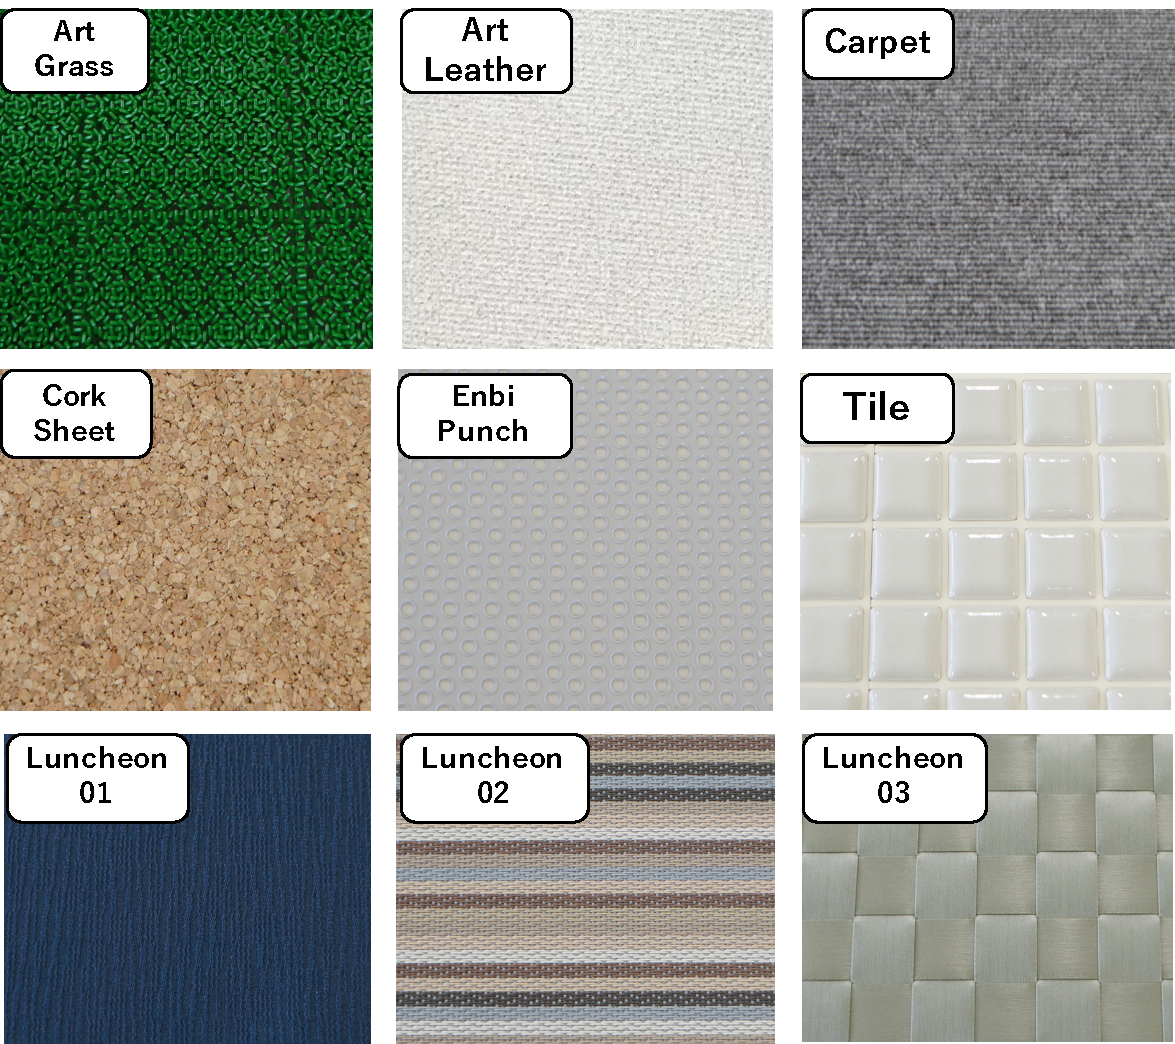
\includegraphics[width=12cm]{eps/textures.pdf}
    \caption{使用した9種のテクスチャ外観}
    \label{fig:texture}
   \end{center}
   \end{figure}

\begin{figure}[H]
    \begin{center}
    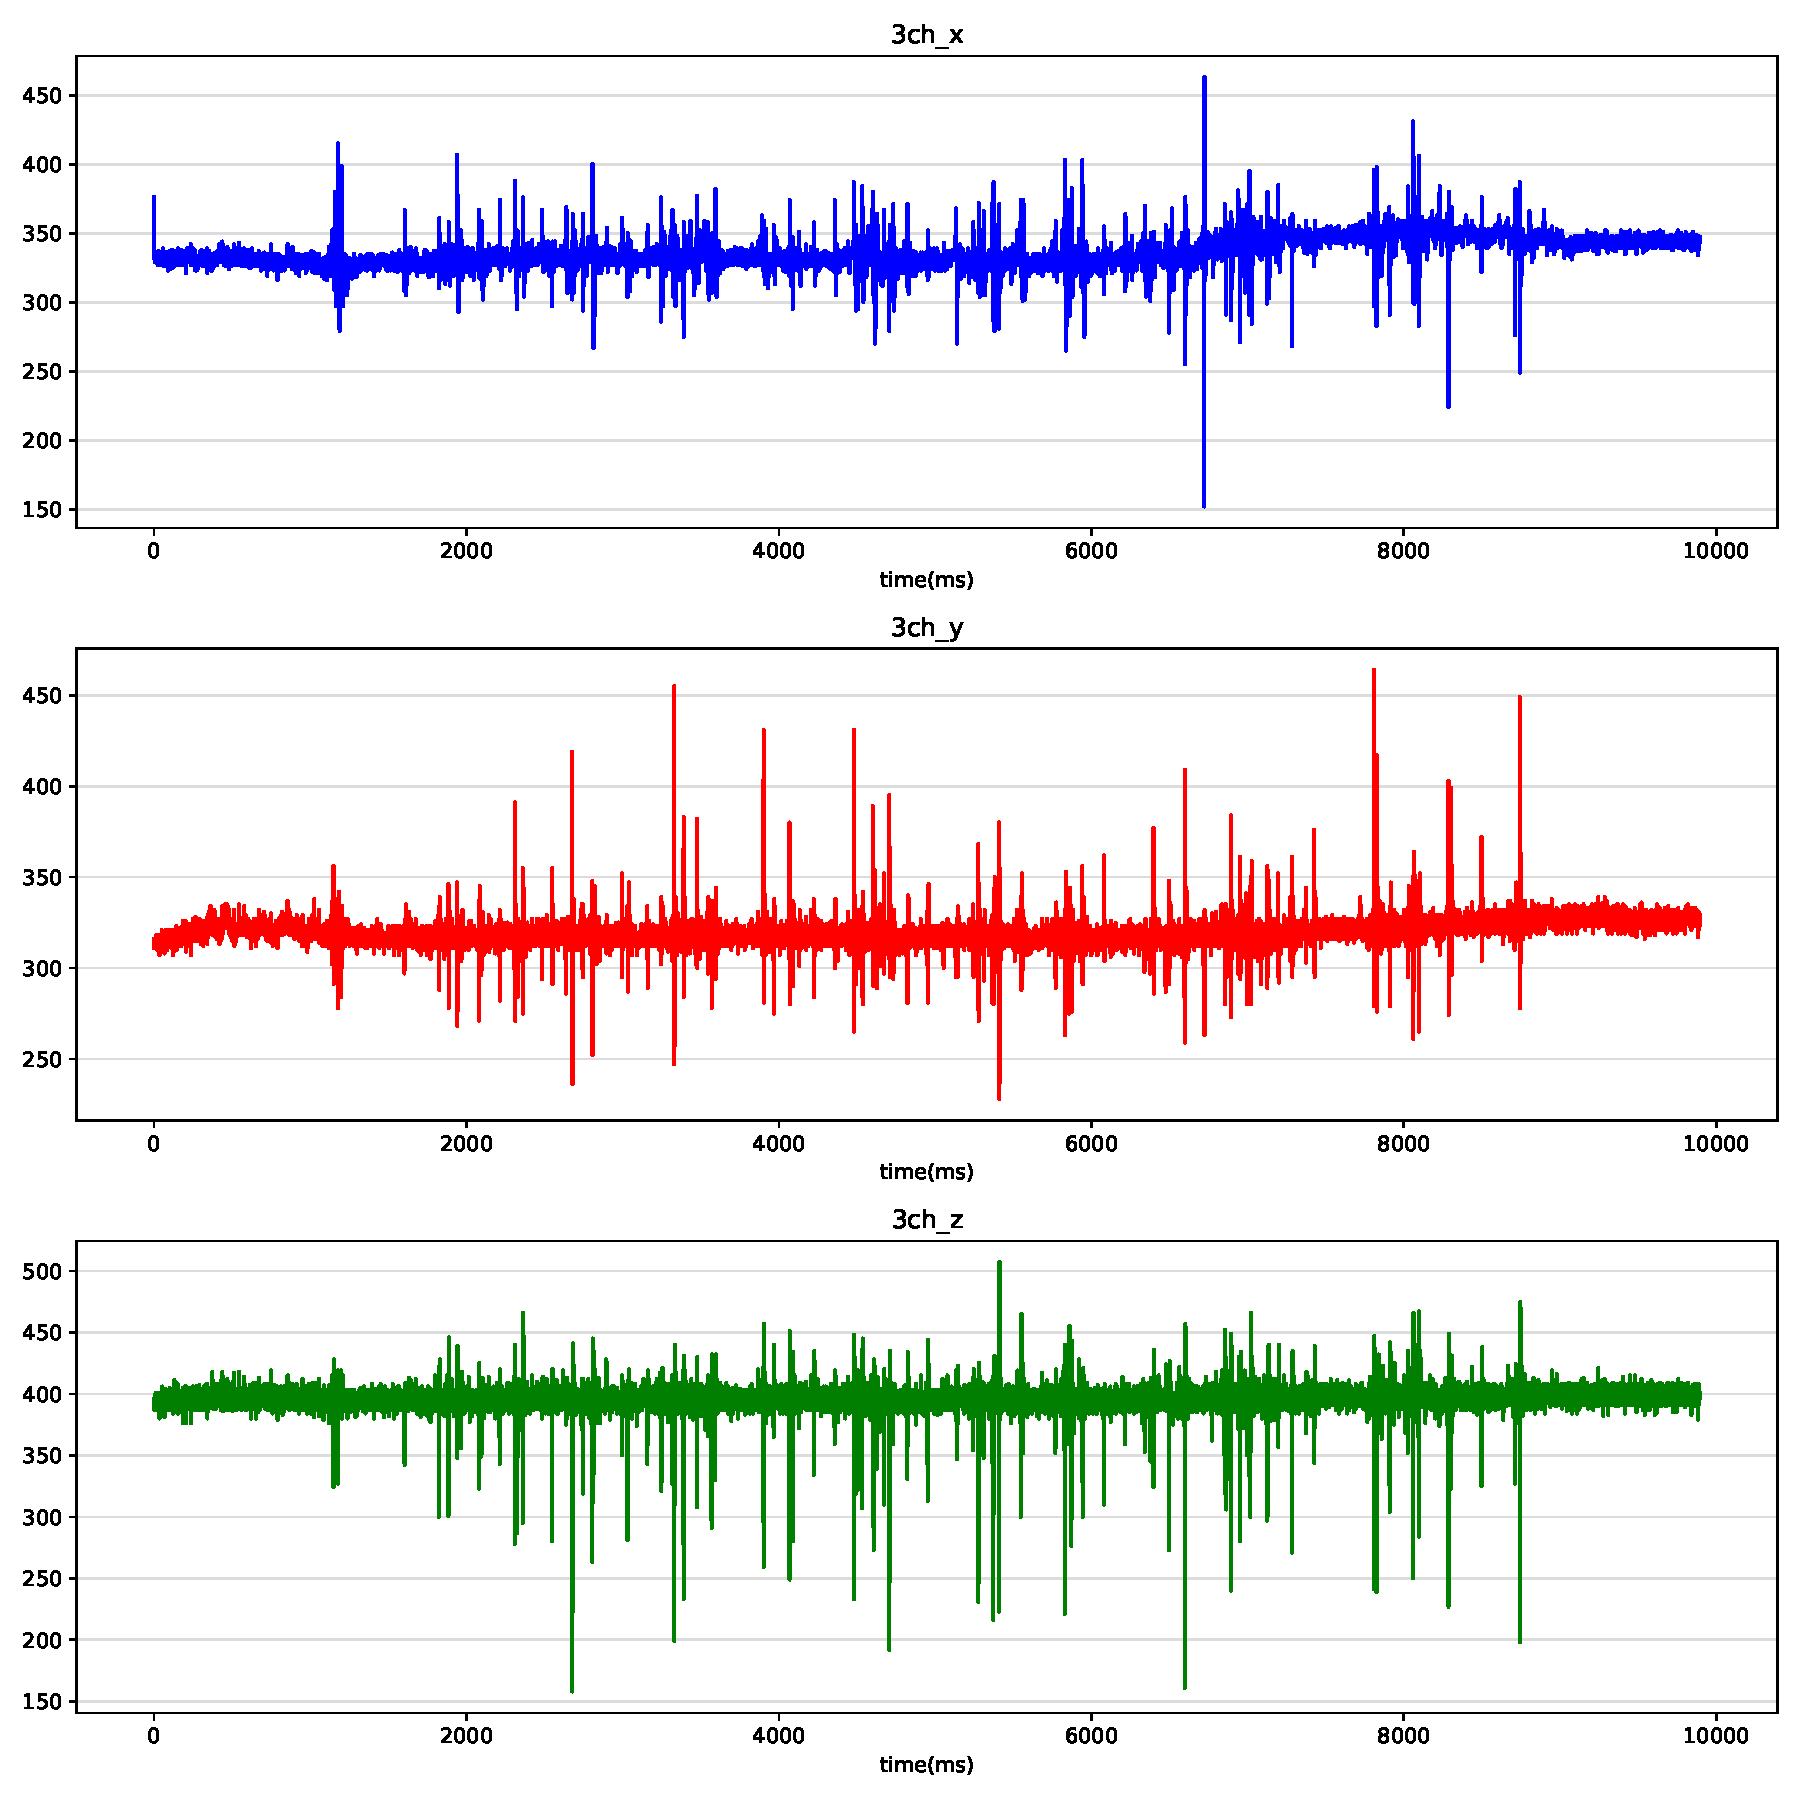
\includegraphics[width=12cm]{eps/3ch.pdf}
    \caption{Art Grass をなぞった際の3軸加速度データ(x,y,z)の例}
    \label{fig:3ch}
   \end{center}
   \end{figure}

\subsection{前処理}
一部の整形したデータは, 比較評価のため上述の各アルゴリズムで次元削減または正規化を行う. 
それぞれの前処理を施した Art Grass をなぞった際の3軸加速度データを各アルゴリズムで次元削減した信号の例を SoC321, Mag321, PCA, DFT321 の順で以下の図\ref{fig:prepros}に示す. 

\begin{figure}[H]
    \begin{center}
    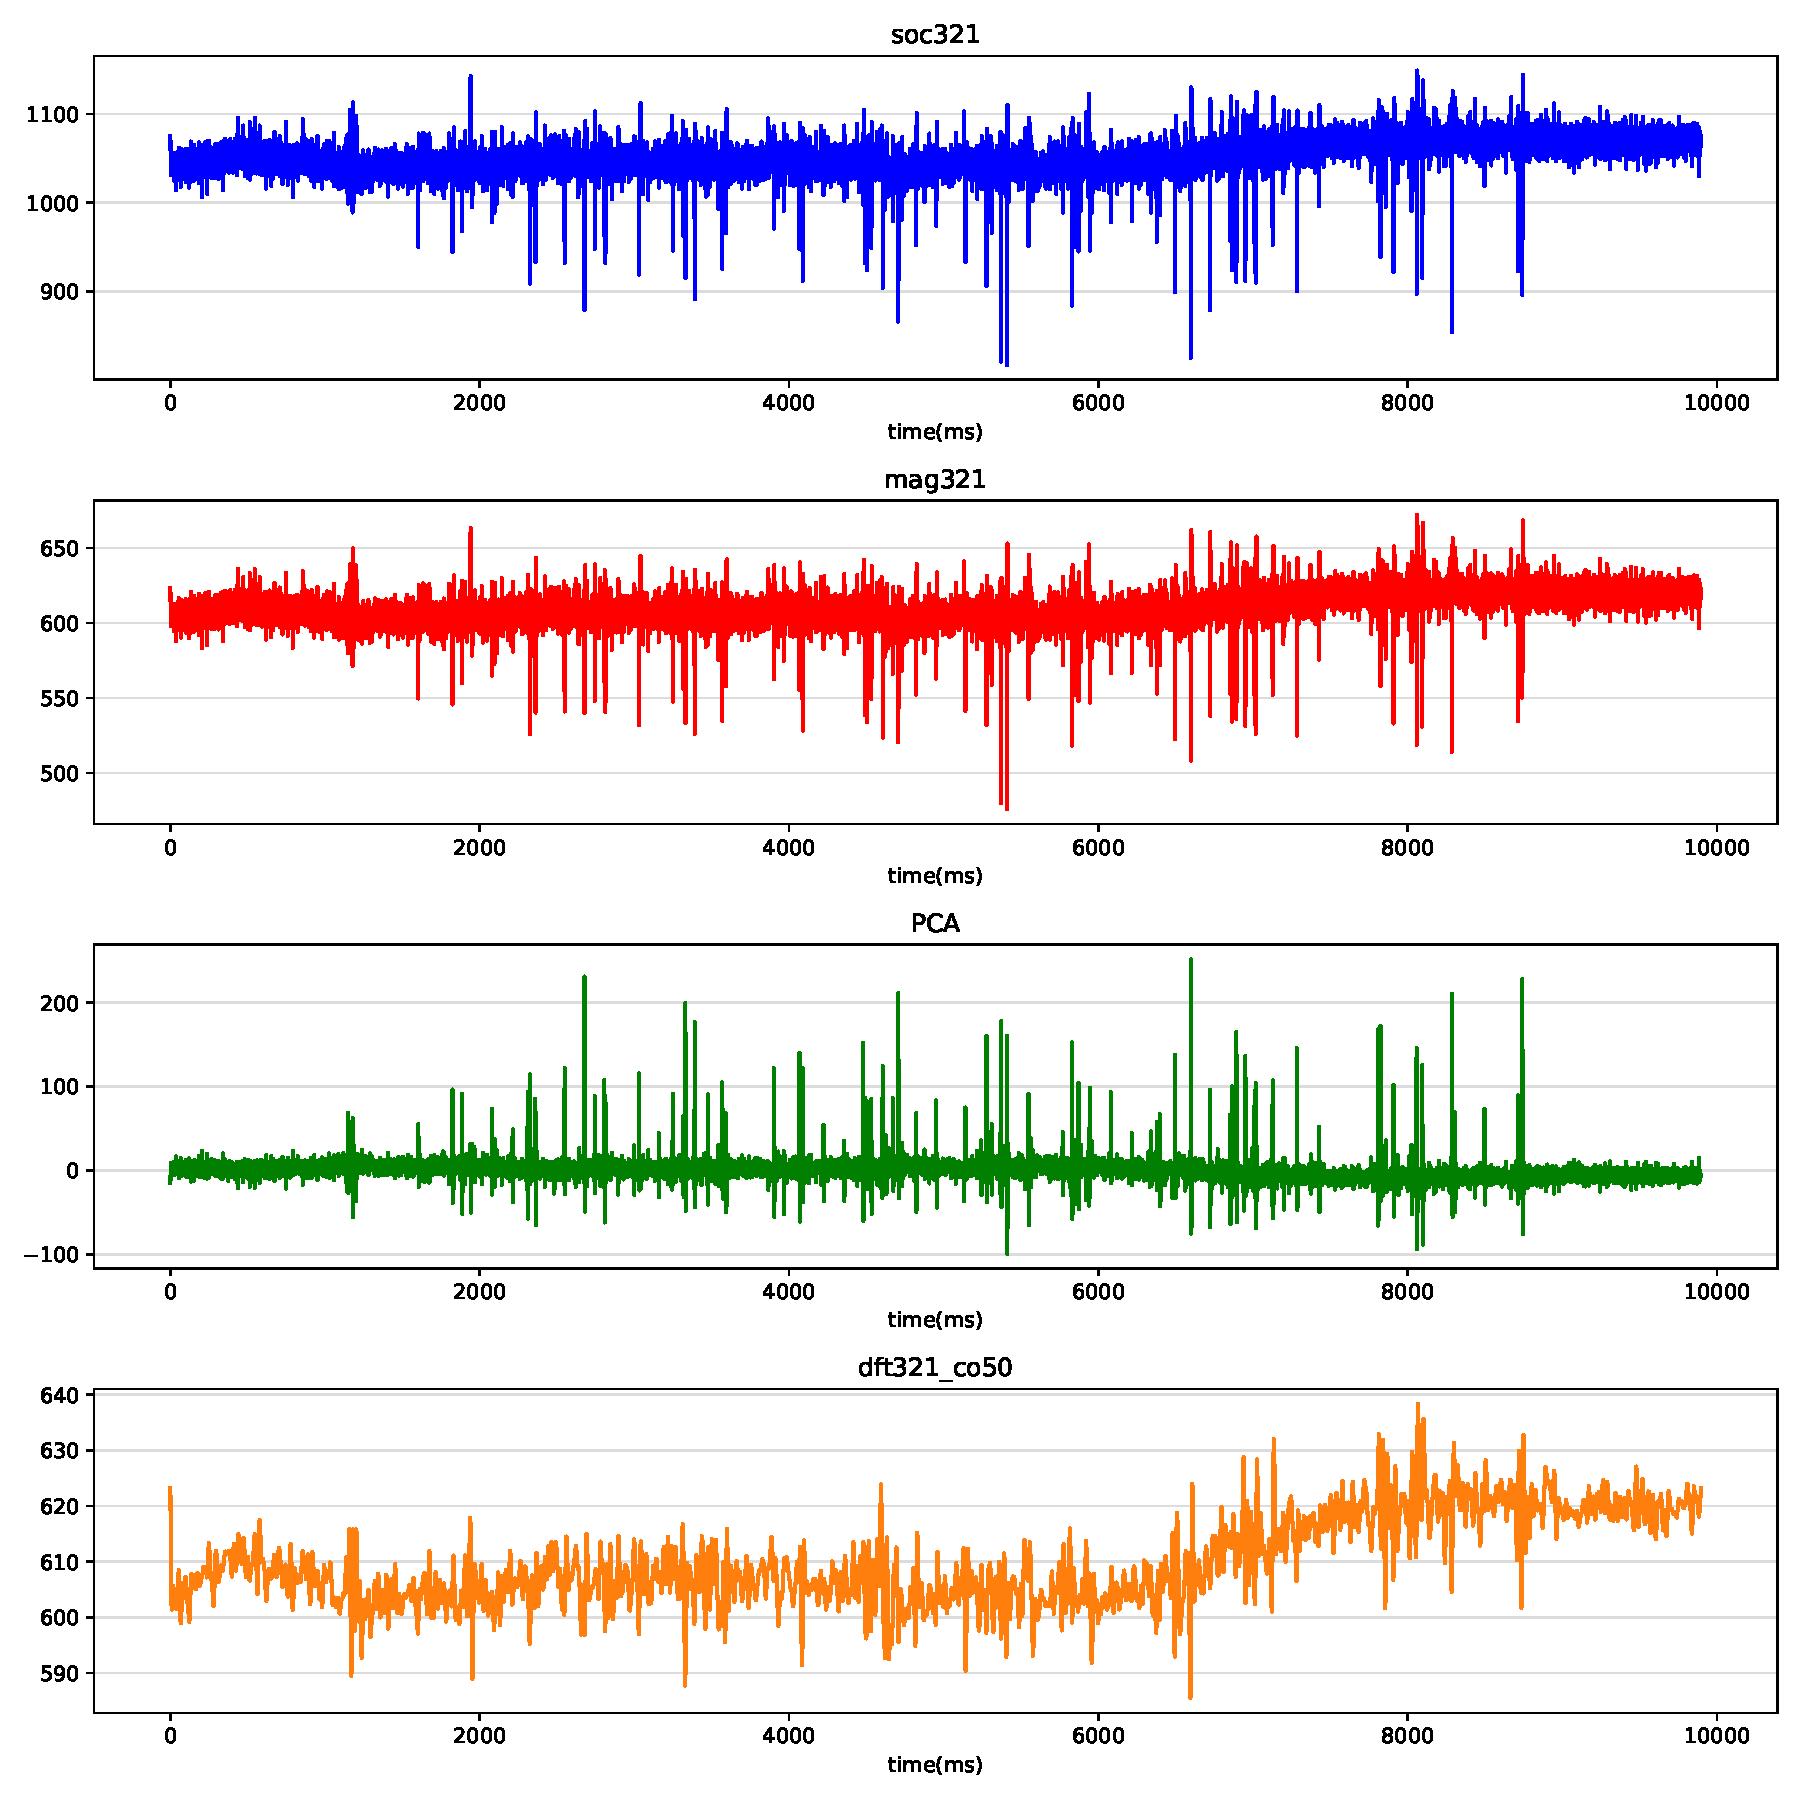
\includegraphics[width=12cm]{eps/1ch_4.pdf}
    \caption{Art Grass をなぞった際の3軸加速度データに各次元削減アルゴリズムを適用した場合の出力信号例}
    \label{fig:prepros}
   \end{center}
   \end{figure}
   
また, 同様に正規化を行った3軸加速度データの信号例を以下の図\ref{fig:normalize}に示す. 

\begin{figure}[H]
    \begin{center}
    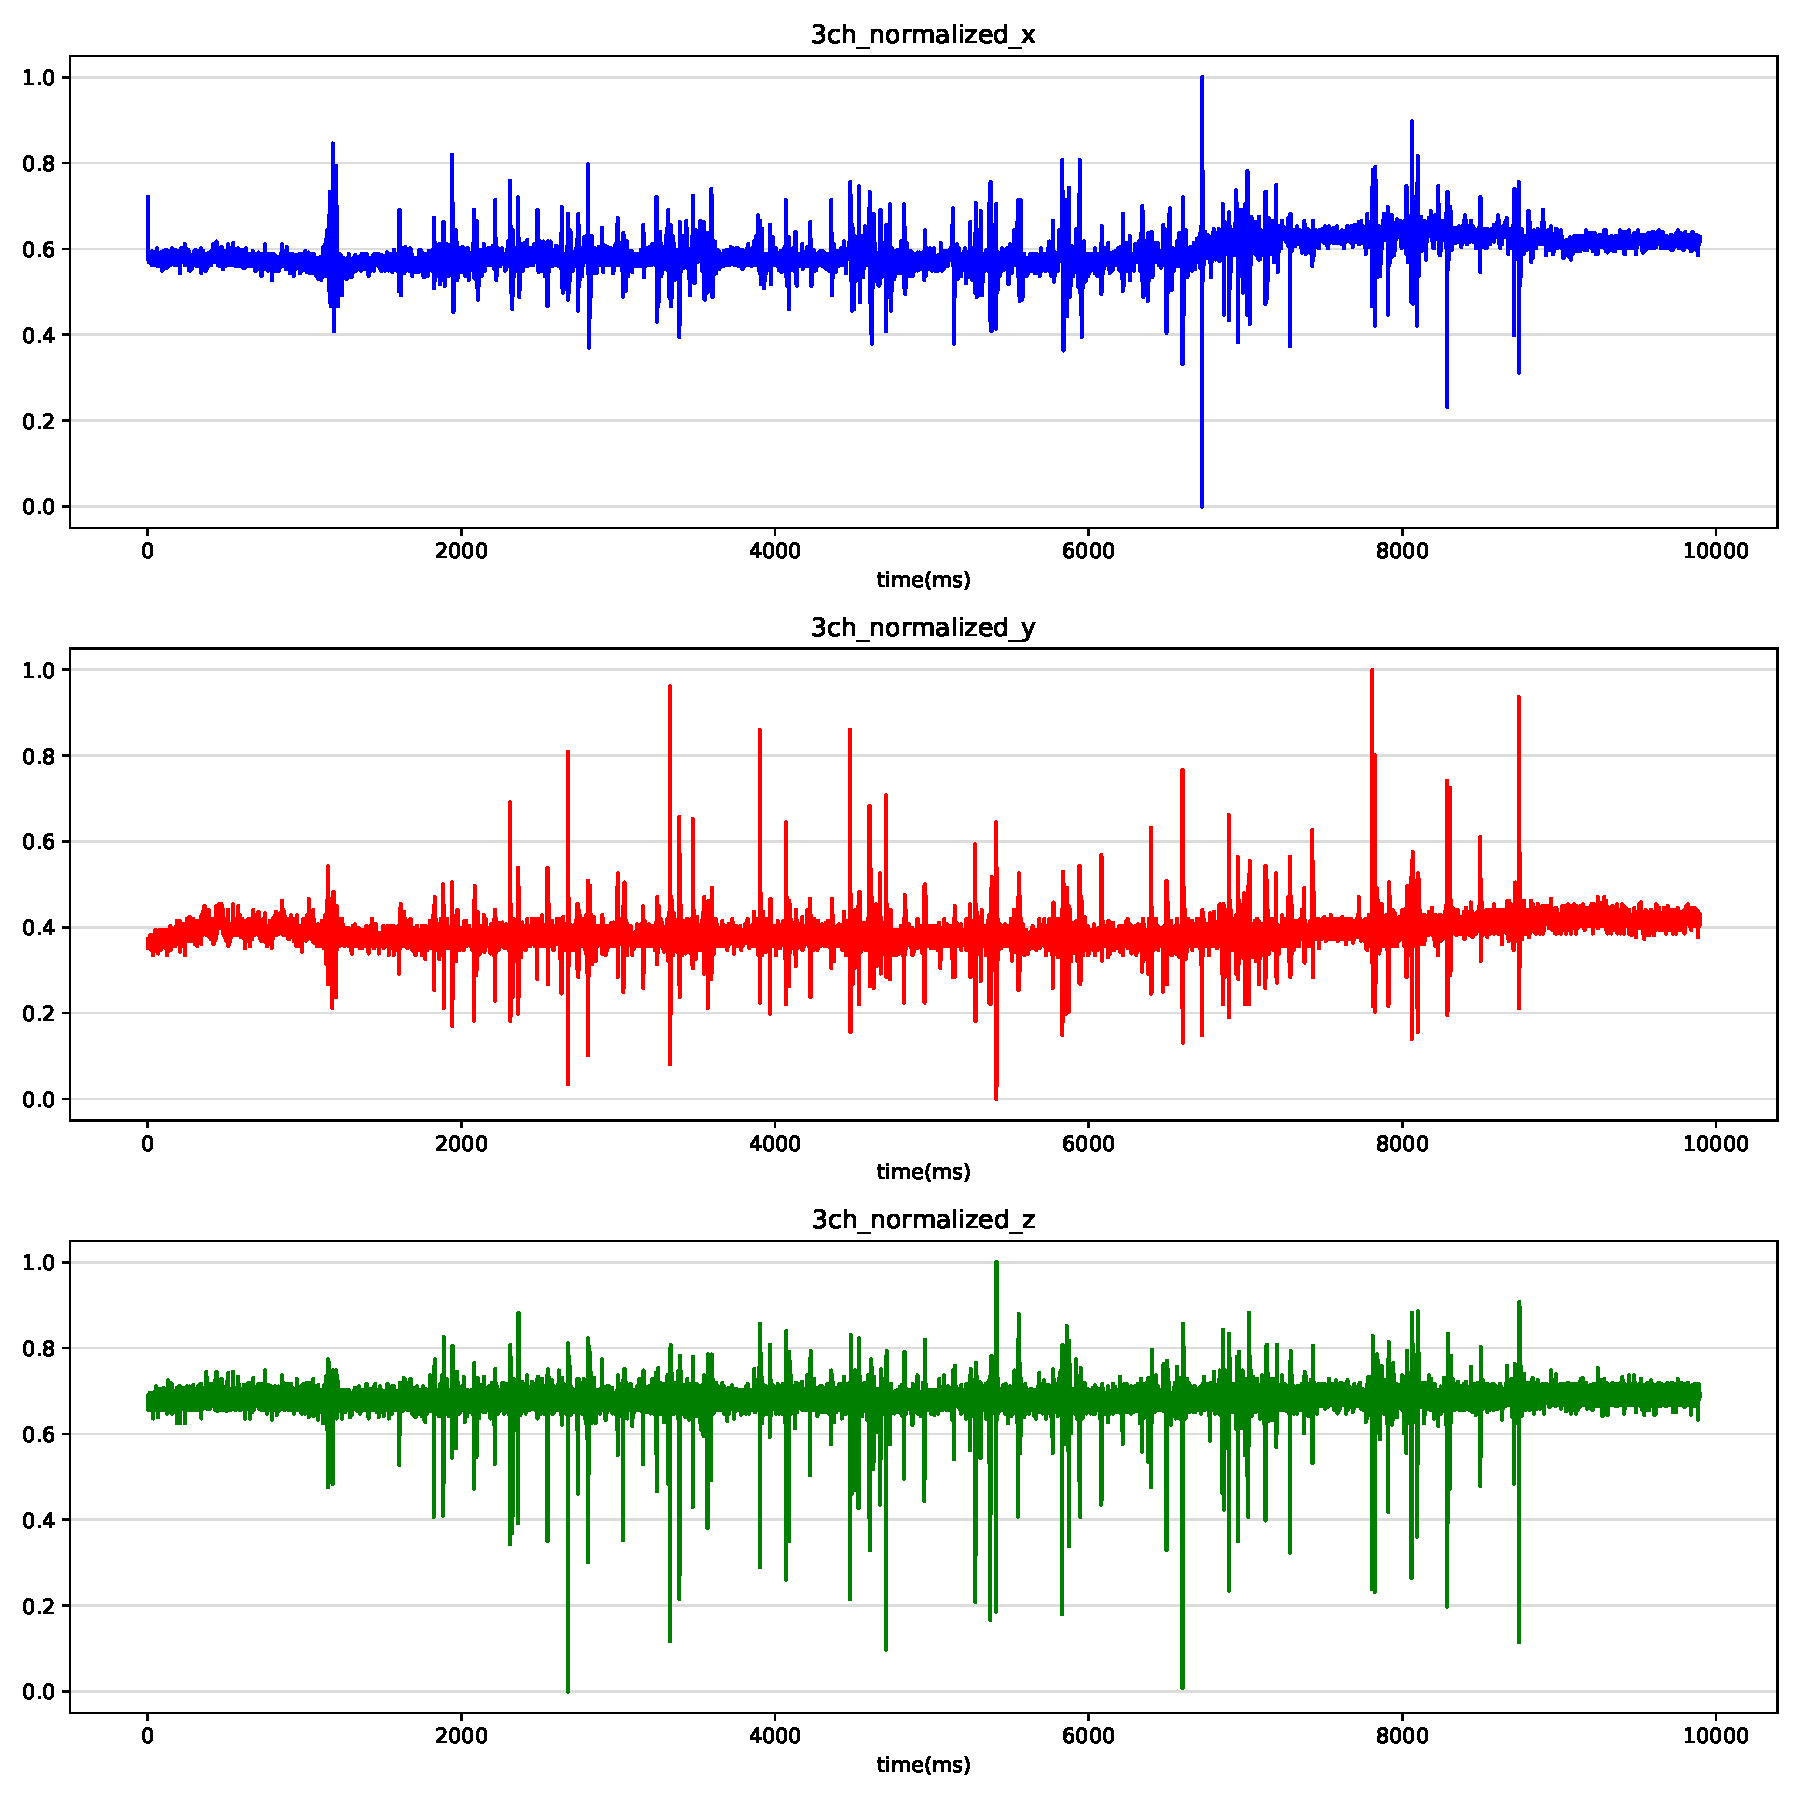
\includegraphics[width=12cm]{eps/3ch_normalized.pdf}
    \caption{Art Grass をなぞった際の3軸加速度データに正規化を適用した場合の出力信号例}
    \label{fig:normalize}
   \end{center}
   \end{figure}
   


\subsection{モデルの構成}
本研究で用いた次元削減信号の分類用 CNN のモデルの構成を以下の表\ref{tab:model_arc}に示す. 前処理にて次元削減を施した時系列加速度データは1次元信号であるので単純にデータ点数 * 1チャネルの入力層を用いる. 次元削減を施さない場合は3軸加速度データなので3チャネルの入力層を用いる. それ以降の構成は同じである. 
畳み込み層の活性化関数$f$として, ReLU関数を用いている. 
活性化関数は入力の総和をどのように発火させ後層に伝達させるかを司る関数である. 
ReLU 関数は負の値をノイズ値として扱う特徴があるが, 勾配消失の少なさと計算量削減の点で他の活性化関数よりも性能が良いとされ, 画像データの処理等で広く使用されている. 
本研究において, 入力の加速度データは負の値を持たないことから ReLU 関数を用いる. 
ReLU 関数は以下の式で定義される. 
\begin{equation}
    f(x)=\left\{\begin{array}{ll}x & (x>0) \\ 0 & (x \leq 0)\end{array}\right.
\end{equation}

\begin{figure}[H]
    \begin{center}
    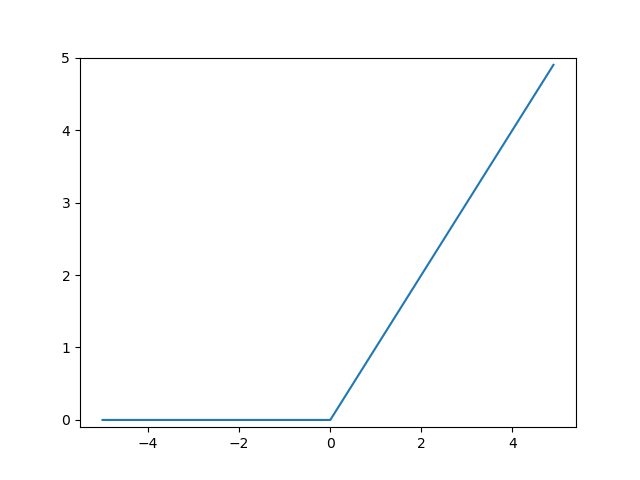
\includegraphics[width=12cm]{eps/relu.png}
    \caption{ReLU関数}
    \label{fig:relu}
   \end{center}
   \end{figure}
   
出力層の手前に全結合層を配置する. 全結合層の出力に活性化関数$f$をかけてモデル全体の出力とする. 
多クラス分類問題において, 出力層の活性化関数にソフトマックス関数を用いた計算が広く使用されている. ソフトマックス関数は以下の式で定義される. 
\begin{equation}
    y_{k}=\displaystyle\frac{\exp \left(a_{k}\right)}{\displaystyle\sum_{i=1}^{n} \exp \left(a_{i}\right)}
\end{equation}
ソフトマックス関数を用いることにより, 出力された値の総和を1に正規化し, ラベルに対する各々の値を確率として捉えることが容易になるという利点がある. 

\begin{table}[H]
\begin{center}
\caption{1次元分類用モデルの構成}
\begin{tabular}{|l||c c c c|c|}
\hline
layer\_name           & filters & kernel\_size & stride & activation & output\_map\_size \\ \hline \hline
input                 & -       & -            & -      & -          & 4096 * 1         \\ \hline
Conv1D\_1             & 64      & 5            & 1      & ReLU       & 4096 * 64          \\ 
Conv1D\_2             & 64      & 5            & 1      & ReLU       & 4096 * 64         \\ 
MaxPooling1D\_1       & -       & 2            & 2      & -          & 2048 * 64         \\ \hline
Conv1D\_3             & 128     & 5            & 1      & ReLU       & 2048 * 128        \\ 
MaxPooling1D\_2       & -       & 2            & 2      & -          & 1024 * 128        \\
Dropout\_1            & -       & -            & -      & -          & 1024 * 128        \\ \hline
Conv1D\_4             & 64      & 5            & 1      & ReLU       & 1024 * 64         \\ \hline
GlobalMaxPooling1D\_1 & -       & -            & -      & -          & 64                \\
Dropout\_2            & -       & -            & -      & -          & 64                \\ \hline
FullyConnected        & -       & -            & -      & Softmax    & 9                 \\ \hline
\end{tabular}
\label{tab:model_arc}
\end{center}
\end{table}

\section{評価指標}
本研究において, 評価実験で得られた出力に対して以下の4つの評価指標とそこから算出する重み付き平均を評価に用いる. 
また, それぞれの指標で用いる TP, TN, FP, FN を以下の表\ref{tab:def_conf}に示す. 

\begin{table}[H]
\begin{center}
\caption{TP, TN, FP, FNの定義}
\begin{tabular}{|c|c|c|c|}
\hline
\multicolumn{2}{|c|}{\multirow{2}{*}{}} & \multicolumn{2}{c|}{Actual}                     \\ \cline{3-4} 
\multicolumn{2}{|c|}{}                  & positive               & negative               \\ \hline
\multirow{2}{*}{predicted}  & positive  & True Positives ( TP )  & False Positives ( FP ) \\ \cline{2-4} 
                            & negative  & False Negatives ( FN ) & True Negatives ( TN )  \\ \hline
\end{tabular}
\label{tab:def_conf}
\end{center}
\end{table}

\begin{itemize}
  \item 精度( Accuracy )
 
  予測結果全体と, 正解ラベルの値がどれぐらい一致しているかを示す. 
  \begin{equation}
    {  Accuracy =\frac{T P+T N}{T P+F P+F N+T N}}
  \end{equation}
  \item 適合率 ( Precision )
  
  あるクラスにおいて, 予測されたもののうち, そのクラスの正解ラベルを有しているものの割合を示す. 
  \begin{equation}
     {  Precision =\frac{T P}{T P+F P}}
  \end{equation}
  \item 再現率 ( Recall )
  
   あるクラスにおいて, 正解ラベルを有しているものうち, 予測でそのクラスに分類されたものの割合を示す. 
  \begin{equation}
     {  Recall =\frac{T P}{T P+F N}}
  \end{equation}
  \item F値 ( $F-measure$ )
  
  トレードオフの関係にある適合率と再現率について両者の調和平均を示す. 
  \begin{equation}
     { F-measure =\frac{2 \cdot  Recall.Precision }{ Recall+Precision }}
  \end{equation}
\end{itemize}

上記の4つの評価指標は, 判別された各クラスに対して値が決まる. したがって9種のクラス分類を行う本研究ではモデルに対して評価指標が噴出し正確な評価につながらない事が考えられる. そこで重み付き平均を導入する. これは多クラスそれぞれのデータ件数の比率を重みとして上記4つのスコア平均を計算する. 
\begin{equation}
    {weighted  X =\frac{\sum w_{i} x_{i}}{\sum w_{i}}}
\end{equation}


% Local Variables:
% TeX-master: "main"
% mode: yatex
% End:
